% documentclass options:
\documentclass[11pt,
  a4paper,
  parskip=half, % This is some extra vertical space between paragraphs, the suggestion is 2cm which is really ugly, so we use what koma script gives us
  % you can also set it to full for even more space. But there is a bad tex style decision: parskip also changes the spacing between listitems such as
  % enumerate and itemize. For this purpose we include the enumitem package and set itemsep=.5em, of course you can change this
  BCOR=10mm, % BCOR is binding correction
  % if you'd rather have a one sided thesis, add `oneside' to the documentclass
  % onside,
  % ngerman is needed for hyphenation if the thesis contains parts written in German, switch order with english if you write mainly in English.
  % Remember to change order in the babel package (below) as well.
  % Last language is the preferred one.
  ngerman,
  english
  ]{scrbook}
\usepackage[ngerman, english]{babel} % If you write mainly in English change order to ngerman, english. Also change that in the documentclass options above.
% Include of titling must happen before \title etc.
% that's why it's not in setup.tex
\usepackage{titling}
\title{Hi-C interaction matrix correction using ICE in Rust}
\author{Felix Karg}

% Change to your first examiner
% The ~ enables non sentence spacing after a period
\newcommand{\firstexaminer}{Prof.~Dr.~Backofen}
% Change to your second examiner, some undergraduate studies don't have a second examiner
% in this case just comment out the following line
% \newcommand{\secondexaminer}{Prof.~Dr.~Wile E. Coyote}
% Change to your adivers
\newcommand{\advisers}{Joachim Wolff, Dr. Mehmet Tekman} % Wolff & Tekman?

% include all packages and define commands in setup.tex

%------------------------------------------------------------------------------
%       package includes
%------------------------------------------------------------------------------
    % font encoding is set up for pdflatex, for other environments see
    % http://tex.stackexchange.com/questions/44694/fontenc-vs-inputenc
    \usepackage[T1]{fontenc}  % 8-bit fonts, improves handling of hyphenations
    \usepackage[utf8x]{inputenc}
    % provides `old' commands for table of contents. Eases the ability to switch
    % between book and scrbook
    \usepackage{scrhack}

    \usepackage{verbatim}
    \usepackage{verbatimbox}

    % ------------------- layout, default -------------------
    % adjust the style of float's captions, separated from text to improve readabilty
    \usepackage[labelfont=bf, labelsep=colon, format=hang, textfont=singlespacing]{caption}
    % With format = hang your caption will look like this:
    % Figure 1: Lorem ipsum dolor sit amet,
    %           consectetuer adipiscing elit.
    %           Ut purus elit, vestibulum
    % If you instead want
    % Figure 1: Lorem ipsum dolor sit amet,
    % consectetuer adipiscing elit. Ut purus
    % elit, vestibulum
    % change to format=plain
    \usepackage{chngcntr}  % continuous numbering of figures/tables over chapters
    \counterwithout{equation}{chapter}
    \counterwithout{figure}{chapter}
    \counterwithout{table}{chapter}

    % Uncomment the following line if you switch from scrbook to book
    % and comment the setkomafont line
    %\usepackage{titlesec}  % remove "Chapter" from the chapter title
    %\titleformat{\chapter}[hang]{\bfseries\huge}{\thechapter}{2pc}{\huge}
    \setkomafont{chapter}{\normalfont\bfseries\huge}

    \usepackage{setspace}  % Line spacing
    \onehalfspacing
    % \doublespacing  % uncomment for double spacing, e.g. for annotations in correction

    % ------------------- functional, default-------------------
    \usepackage[dvipsnames]{xcolor}  % more colors
    \usepackage{array}  % custom format per column in table - needed on the title page
    \usepackage{graphicx}  % include graphics
    \usepackage{subfig}  % divide figure, e.g. 1(a), 1(b)...
    \usepackage{amsmath}  % |
    \usepackage{amsthm}   % | math, bmatrix etc
    \usepackage{amsfonts} % |
    \usepackage{calc}  % calculate within LaTeX
    \usepackage[unicode=true,bookmarks=true,bookmarksnumbered=true,
                bookmarksopen=true,bookmarksopenlevel=1,breaklinks=false,
                pdfborder={0 0 0},backref=false,colorlinks=false]{hyperref}
    \usepackage{etoolbox} % if-else commands


    %==========================================
    % You might not need the following packages, I only included them as they
    % are needed for the example floats
    % ------------------- functional, custom -------------------
    \usepackage{algorithm,algpseudocode}
    \usepackage{bm}  % bold greek variables (boldmath)
    \usepackage{tikz}
    \usetikzlibrary{positioning}  % use: above left of, etc

    % required for the ToDo list
    \usepackage{ifthen}

    % Improves general appearance of the text
    \usepackage[protrusion=true,expansion=true, kerning]{microtype}
    \usepackage{enumitem}
    % nicer font for pdf rendering
    \usepackage{lmodern}

    % For nicer looking tables
    \usepackage{booktabs}

    % usually you don't need this, just for demonstration of a longer caption
    \usepackage{lipsum}

    % for actual Rust syntax highlighting
    \usepackage{minted}
    % \usemintedstyle{arduino}
    % \usemintedstyle{vs}
    % \usemintedstyle{perldoc}
    \usemintedstyle{pastie} % favourite?

%------------------------------------------------------------------------------
%       (re)new commands / settings
%------------------------------------------------------------------------------
    % ----------------- referencing ----------------
    \newcommand{\secref}[1]{Section~\ref{#1}}
    \newcommand{\chapref}[1]{Chapter~\ref{#1}}
    \renewcommand{\eqref}[1]{Equation~(\ref{#1})}
    \newcommand{\figref}[1]{Figure~\ref{#1}}
    \newcommand{\tabref}[1]{Table~\ref{#1}}
    \newcommand{\coderef}[1]{Code Example~\ref{code:#1}}
    \newcommand{\outref}[1]{Output~\ref{out:#1}}

    % ------------------- colors -------------------
    \definecolor{darkgreen}{rgb}{0.0, 0.5, 0.0}
    % Colors of the Albert Ludwigs University as in
    % https://www.zuv.uni-freiburg.de/service/cd/cd-manual/farbwelt
    \definecolor{UniBlue}{RGB}{0, 74, 153}
    \definecolor{UniRed}{RGB}{193, 0, 42}
    \definecolor{UniGrey}{RGB}{154, 155, 156}


    % ------------------- layout -------------------
    % prevents floating objects from being placed ahead of their section
    \let\mySection\section\renewcommand{\section}{\suppressfloats[t]\mySection}
    \let\mySubSection\subsection\renewcommand{\subsection}{\suppressfloats[t]\mySubSection}



    % ------------------- math formatting commands -------------------
    % define vectors to be bold instead of using an arrow
    \renewcommand{\vec}[1]{\mathbf{#1}}
    \newcommand{\mat}[1]{\mathbf{#1}}
    % tag equation with name
    \newcommand{\eqname}[1]{\tag*{#1}}


    % ------------------- pdf settings -------------------
    % ADAPT THIS
    \hypersetup{pdftitle={\thetitle},
                pdfauthor={\theauthor},
                pdfsubject={Undergraduate thesis at the Albert Ludwig University of Freiburg},
                pdfkeywords={deep learning, awesome algorithm,  undergraduate thesis},
                pdfpagelayout=OneColumn, pdfnewwindow=true, pdfstartview=XYZ, plainpages=false}


    %==========================================
    % You might not need the following commands, I only included them as they
    % are needed for the example floats

    % ------------------- Tikz styles -------------------
    \tikzset{>=latex}  % arrow style


    % ------------------- algorithm ---------------------
    % Command to align comments in algorithm
    \newcommand{\alignedComment}[1]{\Comment{\parbox[t]{.35\linewidth}{#1}}}
    % define a foreach command in algorithms
    \algnewcommand\algorithmicforeach{\textbf{foreach}}
    \algdef{S}[FOR]{ForEach}[1]{\algorithmicforeach\ #1\ \algorithmicdo}

    % line spacing should be 1.5
    \renewcommand{\baselinestretch}{1.5}

    % set distance between items in a list, for more details see the
    % enumitem package: https://www.ctan.org/pkg/enumitem
    \setlist{itemsep=.5em}

    % use ra in your tables to increase the space between rows
    % 1.3 should be fine
    \newcommand{\ra}[1]{\renewcommand{\arraystretch}{#1}}

        % ToDo counters
        \usepackage{ifthen} %für whiledo-Schleife
        \newcounter{todos}
        \setcounter{todos}{0}
        \newcounter{extends}
        \setcounter{extends}{0}
        \newcounter{drafts}
        \setcounter{drafts}{0}
        \newcounter{code}
        \setcounter{code}{0}
        \newcounter{outputs}
        \setcounter{outputs}{0}

        % ------------------- marker commands -------------------
    % ToDo command
        \newcommand{\todo}[1]{\textbf{\textcolor{red}{(TODO: #1)}}\refstepcounter{todos}\label{todo \thetodos}}
        \newcommand{\extend}[1]{\textbf{\textcolor{darkgreen}{(EXTEND: #1)}}\refstepcounter{extends}\label{extend \theextends}}
        % Lighter color to note down quick drafts
        \newcommand{\draft}[1]{\textbf{\textcolor{NavyBlue}{(DRAFT: #1)}}\refstepcounter{drafts}\label{draft \thedrafts}}

        % microtype with lmodern, see https://tex.stackexchange.com/questions/75305/microtype-warning-with-lmodern-package-and-koma-script
        %\DeclareMicrotypeAlias{lmss}{cmr}

        \newenvironment{codeboxed}[1]
                {\nobreak\nobreak\begin{center}#1\\[1ex]\begin{tabular}{|p{\textwidth}|}\hline}
                {\\\hline\end{tabular}\end{center}}

        % (Rust) Code Environment has two variables, the filename and some label.
        \newcommand{\code}[2]{\refstepcounter{code}\label{code:#2}\begin{codeboxed}{Code Example \thecode}
            \inputminted[linenos,fontsize=\small]{Rust}{code/#1}\end{codeboxed}}

        \newcommand{\console}[2]{\refstepcounter{outputs}\label{out:#2}\begin{codeboxed}{Output Nr. \theoutputs}
        {\small\verbatiminput{code/#1}}\end{codeboxed}}

        % \newenvironment{coutput}[1]
        %     {\refstepcounter{outputs}\label{out:#1}\begin{codeboxed}{Output Nr. \theoutputs}\small}
        %     {\end{codeboxed}\normalsize}


        % \newcommand{\todo}[1]{\textbf{\textcolor{red}{(TODO: #1)}}\refstepcounter{todos}\label{todo \thetodos}}




\begin{document}
    \pagestyle{empty} % no header and no page number
    % disable hyper links to remove warning "destination with same identifier"
    % this means within this section nothing can be referenced with a hyperlink
    \hypersetup{pageanchor=false}

    % enable/disable, depending on your chosen language
    
\begin{titlepage}
\begin{center}

\newcommand{\HorizontalLine}{\rule{\linewidth}{0.3mm}}

{\Large Bachelor Thesis}\\[1.3cm]


% _____________________________________________________________________________
\HorizontalLine \\[0.4cm]
% Write your title in a fancy way like this if you want to customize it, otherwise simply let tex do it for you
% \begin{spacing}{3}
%     {\huge \bfseries The Long, Long } \\
%     {\huge \bfseries Long Long} \\
%     {\huge \bfseries Title}\\
% \end{spacing}
{ \huge \bfseries \thetitle }
\HorizontalLine \\[1.5cm]
% _____________________________________________________________________________


{\Huge \theauthor} \\[2cm]


\begin{tabular}[hc]{>{\huge}l >{\huge}l}
  Examiner: & \firstexaminer \\[0.3cm]
  Advisers: & \advisers \\[1.2cm]
\end{tabular}
\vfill  % move the following text to the bottom

\Large {
    Albert-Ludwigs-University Freiburg\\
    Faculty of Engineering\\
    Department of Computer Science\\
    Chair for Bioinformatics\\[1cm]

    July 10\textsuperscript{th}, 2019\\
}
\end{center}
\end{titlepage}

\thispagestyle{empty}
\ \vfill \ \\
\newpage
\thispagestyle{empty}
% title page back
\ \vfill \ \\  % at least one space required before vfill
\
\textbf{Writing Period}            \smallskip{} \\
10.\,04.\,2019 -- 10.\,07.\,2019   \bigskip{} \\
\
\textbf{Examiner}                  \smallskip{} \\
\firstexaminer                     \bigskip{} \\
\
% If there is a second examiner include it
\ifdef{\secondexaminer}
	{
	% Include
	\textbf{Second Examiner}       \smallskip{} \\
	\secondexaminer                \bigskip{} \\
	\
	}
	{
	% No second examiner, ignore
	}
\textbf{Advisers}                  \smallskip{} \\
\advisers

\newpage
\thispagestyle{empty}
\ \vfill \ \\

    % % \begin{titlepage}
\begin{center}

\newcommand{\HorizontalLine}{\rule{\linewidth}{0.3mm}}

{\Large Bachelor Thesis}\\[1.3cm]


% _____________________________________________________________________________
\HorizontalLine \\[0.4cm]
% Write yourtitle in a fancy way like this if you want to customize it, otherwise simply let tex do it for you
% \begin{spacing}{3}
%     {\huge \bfseries Der Lange, Lange } \\
%     {\huge \bfseries Lange Lange} \\
%     {\huge \bfseries Titel}\\
% \end{spacing}
{ \huge \bfseries \thetitle }
\HorizontalLine \\[1.5cm]
% _____________________________________________________________________________


{\Huge \theauthor} \\[2cm]


\begin{tabular}[hc]{>{\huge}l >{\huge}l}
  Gutachter: & \firstexaminer \\[0.3cm]
  Betreuer: & \advisers \\[1.2cm]
\end{tabular}
\vfill  % move the following text to the bottom

\Large {
    Albert-Ludwigs-Universität Freiburg\\
    Technische Fakultät\\
    Institut für Informatik\\
    Lehrstuhl für Bioinformatik\\[1cm]

    10. Juli 2019
    \\
}
\end{center}
\end{titlepage}

\thispagestyle{empty}
% title page back
\ \vfill \ \\  % at least one space required before vfill
\
\textbf{Bearbeitungszeit}            \smallskip{} \\
10.\,04.\,2016 -- 10.\,07.\,2016   \bigskip{} \\
\
\textbf{Gutachter}                  \smallskip{} \\
\firstexaminer                      \bigskip{} \\
\
% If there is a second examiner include it
\ifdef{\secondexaminer}
	{
	% Include
	\textbf{Zweitgutachter}        \smallskip{} \\
	\secondexaminer                \bigskip{} \\
	\
	}
	{
	% No second examiner, ignore
	}
\textbf{Betreuer}                  \smallskip{} \\
\advisers


    \pagestyle{plain} % remove chapter name from top, page number at the bottom
    % use \pagestyle{headings} for having the chapter on top of the pages
    % if you wang a more fancy header use \usepackage[automark,headsepline]{scrlayer-scrpage}
    % and read about it in the KOMA script documentation, https://www.ctan.org/pkg/koma-script
    \frontmatter  % roman page numbers
    % official declaration from the examination office; to be sure double
% check the wording on their website
% (https://www.tf.uni-freiburg.de/studies/exams/thesis/thesis_formatting.html#erklaerung)

% \section*{Erklärung}
\chapter*{Erklärung}

Hiermit erkläre ich, dass ich diese Abschlussarbeit selbständig verfasst habe, keine anderen
als die angegebenen Quellen/Hilfsmittel verwendet habe und alle Stellen, die wörtlich oder
sinngemäß aus veröffentlichten Schriften entnommen wurden, als solche kenntlich gemacht
habe. Darüber hinaus erkläre ich, dass diese Abschlussarbeit nicht, auch nicht
auszugsweise, bereits für eine andere Prüfung angefertigt wurde.
\\[3\normalbaselineskip]
\begin{tabular}{p{\textwidth/2} l}
  \rule{\textwidth/3}{0.4pt}   &   \rule{\textwidth/3}{0.4pt} \\
  Ort, Datum                   &   Unterschrift
\end{tabular}
\newpage

% \section*{Declaration}
%
% I hereby declare, that I am the sole author and composer of my thesis and that no other sources or learning aids, other than those listed, have been used. Furthermore, I declare that I have acknowledged the work of others by providing detailed references of said work.  \newline
% I hereby also declare, that my Thesis has not been prepared for another examination
% or assignment, either wholly or excerpts thereof.
% \\[3\normalbaselineskip]
% \begin{tabular}{p{\textwidth/2} l}
%   \rule{\textwidth/3}{0.4pt}   &   \rule{\textwidth/3}{0.4pt} \\
%   Place, Date                  &   Signature
% \end{tabular}



    \chapter*{Abstract}

foo




\todo{Write!}






\chapter*{Zusammenfassung}

bar






\todo{Schreiben!}

    \tableofcontents
    \listoffigures
    % \listoftables
    % \listofalgorithms
    \hypersetup{pageanchor=true}  % re-enable hyperlinking

    \mainmatter  % Arabic page numbers
    \chapter{Introduction}\label{chap:introduction}

Hi-C is a method commonly used for getting 3D-information of genomes. Such
technologies tend to suffer from technical (e.g. sequencing, mapping)
\cite{pmid21646344} and biological factors (e.g. distinct chromatin states)
\cite{pmid19693276}, making them inherently inaccurate.

However, a basic assumption about the structure of the genome can be made,
which is that every location has the same amount of interactions (with other
locations) as every other location. The data does not show this due to the
several aforementioned inaccuracies. Algorithms such as ICE (Iterative
Correction and Eigenvector decomposition, \secref{sec:ICE}) or KR (Knight-Ruiz,
\secref{sec:KR}) can be applied to ``normalize'' the matrix nonetheless.

ICE, the algorithm implemented in this work, ``normalizes'' the data we
have iteratively. Eigenvector decomposition of the normalized data can then
give us new insights on local chromatin states or global patterns of
chromosomal interaction \cite{imakaev2012iterative}.

We will not do the Eigenvector decomposition, but the iterative correction
(``normalization'') before that.


\section{Core setup}\label{sec:setup}

This work is part of the HiCExplorer (\secref{sec:hicexplorer}) tool from the
Deeptools (\secref{sec:deeptools}) framework. HiCExplorer is mainly written in
Python, being limited by the high resource requirements of the iteration process.

% As we will see, the implementation in rust is faster even when using only one core.

\todo{run experiments!!}


% with this implementation needing too much working memory (RAM) for the
% iterative correction. For some time, the goal was to reduce memory usage by not
% copying a huge matrix a couple of times. From the Rust side, it would have been
% possible to read and write to the matrix in-memory, but we decided against
% doing so due to concerns regarding correctness. Still, the focus is to
% investigate which version requires less resources (CPU Time/RAM/...).


% This is going to be an interesting comparison, since, the (before) default
% Python-implementation was only using one core. Rust code written for
% single-core applications can easily be turned to multicore code. During the
% work of this project, an implementation of a different algorithm
% (\secref{sec:KR}) written in C++ got added, so We'll compare with this one now
% as well.

\extend{Add more details!!}


\section{Algorithm}\label{sec:algorithm}

% Wolff: Jede Position im Genom hat in der Summe die gleiche anzahl an
%        interaktionen mit anderen Positionen des Genoms.

Fundamentally, every part in our genome has the same amount of summed up
interactions with other parts of the genome. The algorithm takes severe
advantage of this property, downright enforcing it. A full description can be
found in \secref{sec:ICE}.



\section{Motivation}\label{sec:motivation}

\subsection{Motivation for Hi-C}

Within cells, the three-dimensional structure of chromatin can now be analyzed
using techniques based on chromatin conformation capture (C3), including Hi-C.
With Hi-C \draft{what is the long name?}, we can construct spatial proximity
maps over the whole genome, giving us clues as to which regions are close to
each other. With C3 it can be tested if two genomic locations are close to each
other, but with Hi-C we get (biased but still) all spatial connections of the
genome at once.

\subsection{Motivation for Rust}

There is several reasons for using Rust, including faster development than C++
and better tooling, while still having the same if not slightly better
performance. A massive advantage is the easiness of adding parallelism, and the
modularity of Rust code. Libraries in Rust can easily be stacked, and the
compiler will complain if the memory is not handled the way it should be (in
C++ it is hard to correctly manage all memory, especially from libraries,
easily resulting in segfaults and similar issues hard to debug). The benefits to
using Rust instead of Python are only apparent if performance or safety (of
execution, at runtime) is needed - which is the case here.





    \chapter{Background}\label{chap:background}
% \begin{algorithm}[p]
\caption{Stochastic Gradient Descent: Neural Network}
\label{alg:backpropnn}
\begin{algorithmic}
    % \ttfamily
    \State Create a mini batch of $m$ samples $\vec{x}_0 \ldots \vec{x}_{m-1}$
    \ForEach{sample $\vec{x}$}
        \State $\vec{a}^{\vec{x},0} \gets \vec{x}$  \alignedComment{Set input activation}
        \ForEach{Layer $l \in \{1\ldots L-1\}$}  \alignedComment{Forward pass }
            \State $\vec{z}^{\vec{x},l} \gets \mathbf{W}^l \vec{a}^{\vec{x},l-1}+\vec{b}^l$
            \State $\vec{a}^{\vec{x},l} \gets \varphi(\vec{z}^{\vec{x},l})$
        \EndFor
        \State $\bm{\delta}^{\vec{x},L} \gets \nabla_{\vec{a}} C_\vec{x} \odot \varphi'(\vec{z}^{\vec{x},L})$ \alignedComment{Compute error}
        \ForEach{Layer $l \in L-1, L-2 \ldots 2$}  \alignedComment{Backpropagate error}
            \State $\bm{\delta}^{\vec{x},l} \gets ((\mathbf{W}^{l+1})^T \bm{\delta}^{\vec{x},l+1})\odot \varphi'(\vec{z}^{\vec{x},l})$
        \EndFor
    \EndFor
    \ForEach{$l \in L, L-1 \ldots 2$} \Comment  \alignedComment{Gradient descent}
        \State $ \mathbf{W}^l \gets \mathbf{W}^l-\frac{\eta}{m} \sum_\vec{x} \bm{\delta}^{\vec{x},l} (\vec{a}^{\vec{x},l-1})^T$
        \State $\vec{b}^l \gets \vec{b}^l-\frac{\eta}{m}\sum_\vec{x} \bm{\delta}^{\vec{x},l}$  
    \EndFor
\end{algorithmic}
\end{algorithm}
% 
%
% \begin{figure}[t]
%     \begin{center}
%     \begin{tikzpicture}
%         \node (a) at (0,0) {a};
%         \node (b) at (2, 0) {b};
%         \draw[->] (a) -- (b);
%
%
%     \end{tikzpicture}
%     \end{center}
%     \caption[Tikz Example]{Use tikz to draw nice graphs!}
%     \label{fig:Tikz}
% \end{figure}


\section{Chromosome Conformation Capture and Hi-C}\label{sec:c3}\label{sec:hic}

\begin{figure}[t]
\begin{centering}
%    \subfloat[Diagram summarising the Hi-C experimental protocol. The red and blue rectangles represent cross-linked restriction fragments while the yellow marker shows the position of biotin incorporation.]
%    \subfloat[Generation of the Hi-C ligation junction sequence by successive digestion (with HindIII in this example), fill in and blunt-ended ligation steps. The modified restriction site sequence is not found in the original genomic sequence.]
    {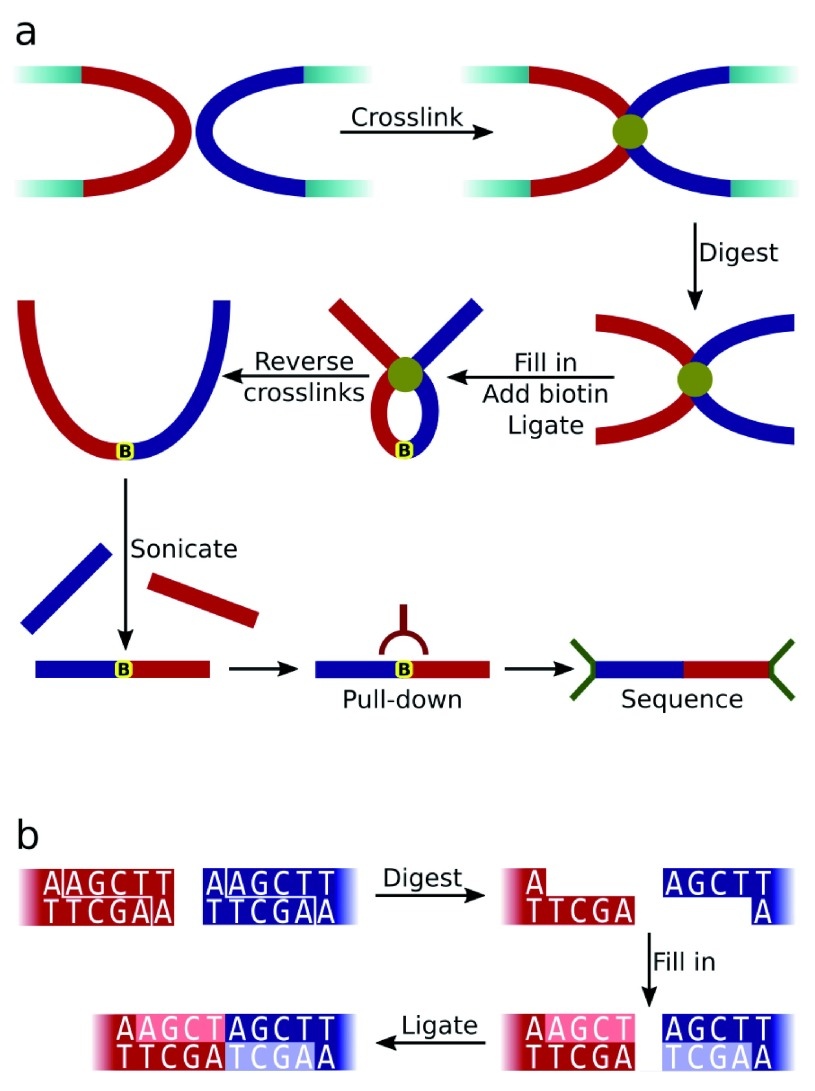
\includegraphics[scale=4]{figures/background/f1000research-4-7903-g0000.jpg}}
    \caption[Summarised Hi-C protocol]
    {\textbf{a)} Diagram summarising the Hi-C experimental protocol. The red and blue rectangles represent cross-linked restriction fragments while the yellow marker shows the position of biotin incorporation. \textbf{b)} Generation of the Hi-C ligation junction sequence by successive digestion (with HindIII in this example), fill in and blunt-ended ligation steps. The modified restriction site sequence is not found in the original genomic sequence. \\ \\ Image and description taken from \cite{wingett2015hicup}.}
    \label{fig:HiC}
    \todo{rewrite the description in my own words}

    \todo{remove the b section}
\end{centering}
\end{figure}



    % {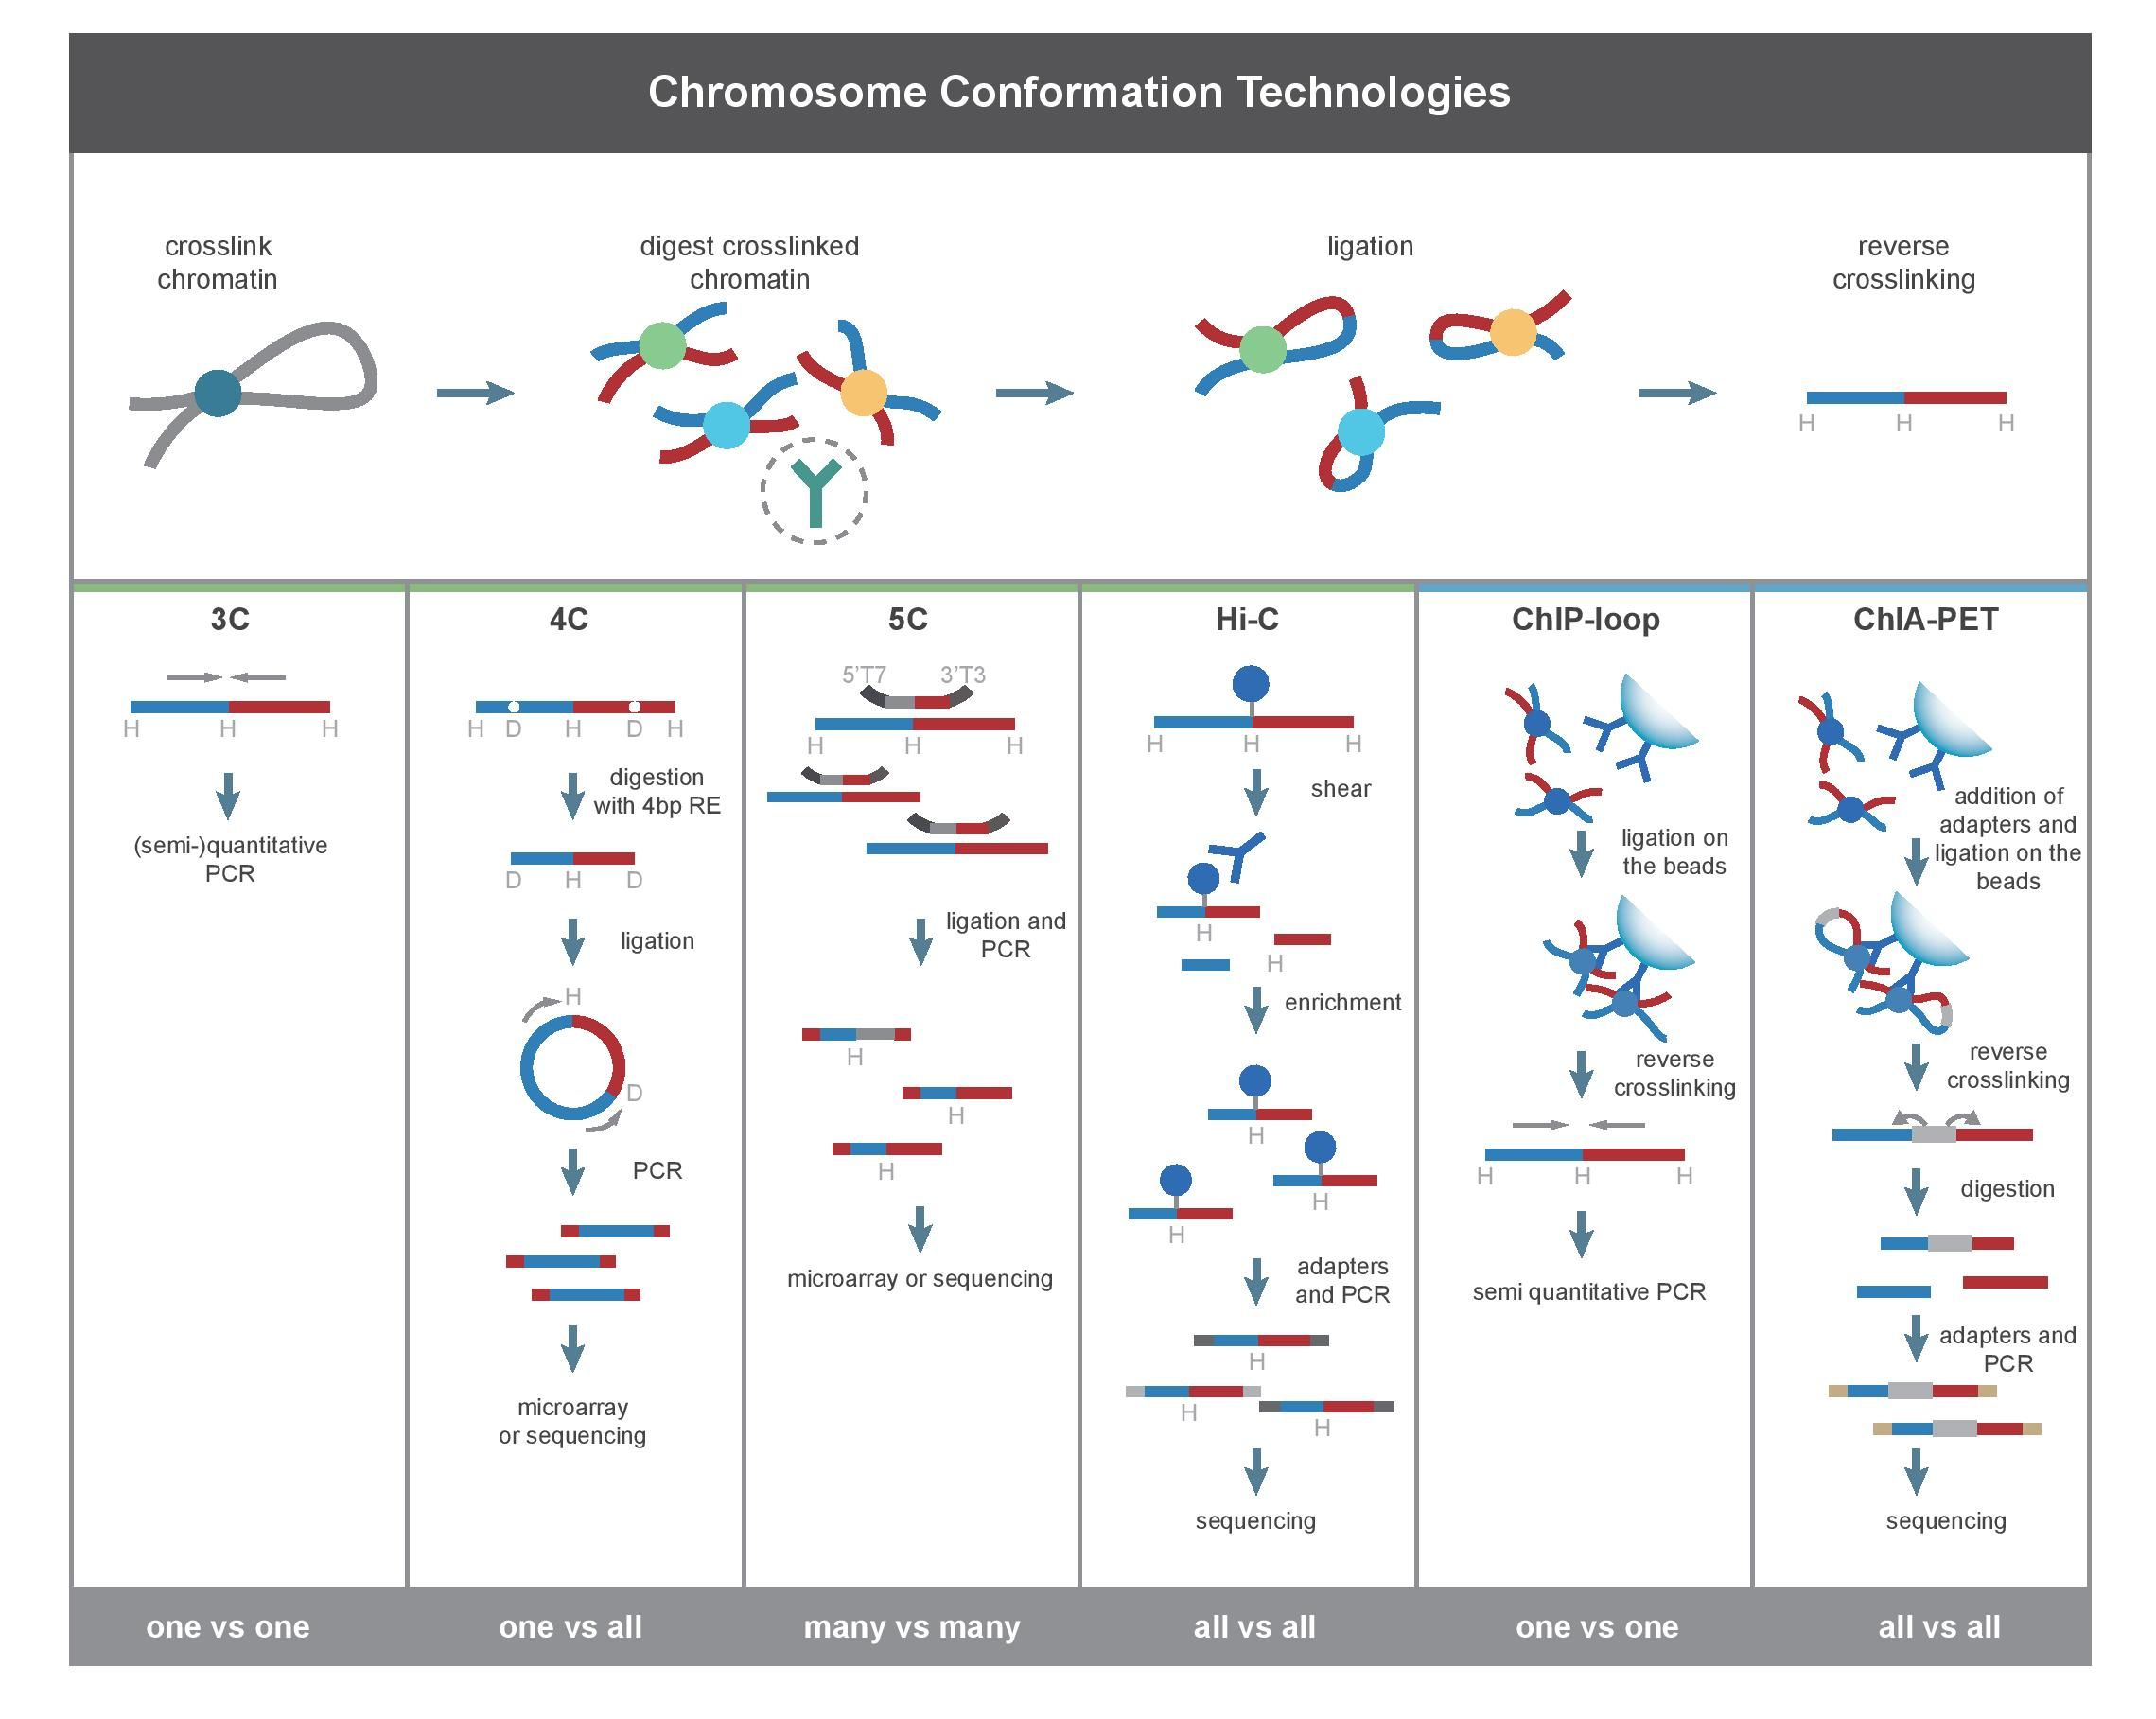
\includegraphics[scale=0.8]{figures/background/Chromosome_conformation_techniques.jpg}}
    % \caption[Comparison among 3C and its derived methods]{\textbf{Comparison among 3C and its derived methods} Source: https://en.wikipedia.org/wiki/File:Chromosome\_conformation\_techniques.jpg}


\subsection{Overview}


Chromatin usually describes different levels of how DNA organizes itself. The
well-known double-helix is only the lowest of several structural layers.

Looking at it from the outside (highest structural layer), DNA looks similar to
a big ball of wool. With the help of Hi-C (or other methods) we can visualize
the spatial proximity.

% Gene markers tend to also have effect on their spatial neighbourhood, not only on the neighbourhood going up and down the strand of DNA.



Chromosome Conformation Technologies describe several similar methods to
compare genomic loci. They all start by:

\begin{itemize}
    \item creating chromatin cross-links (\secref{sec:crosslinking}),
    \item digesting the cross-linked chromatin (\secref{sec:digestion}),
    \item ligating the ends and marking with Biotin (\secref{sec:ligation}) and
    \item reversing the cross-link (\secref{sec:revcrosslink})
\end{itemize}

to get a sequence with two parts, those parts have been spatially close
to each other and were marked with Biotin during ligation.

Other Chromosome Conformation Technologies proceed differently, Hi-C, our
focus, continues with the following steps:

\begin{itemize}
    \item shortening the cross-links by sonication (\secref{sec:sonication}),
    \item filtering leaving only those with biotin (\secref{sec:pulldown}) and
    \item sequencing (\secref{sec:sequencing}).
\end{itemize}

The full process can be seen in \figref{fig:HiC}.

\subsection{Cross-linking DNA}\label{sec:crosslinking}

The first step is to cross-link DNA strands that are close to each other
spatially (see \figref{fig:HiC} for reference). This is done by adding
formaldehyde, which bonds (links) sufficiently close strands together.

A chromatin cross-link is two entirely different parts of the genome held
together by a chemical bond with formaldehyde. This process cannot be
specifically controlled, so only `regions near each other' are connected, not
necessarily two `known to be close' regions.

\subsection{Digestion}\label{sec:digestion}

The next step is cutting the ball of wool apart in intervals. For this,
restriction-enzymes are used (specifically restriction endonuclease). Commonly
used enzymes for this are EcoR1 or HindIII, cutting the genome every 4000 base-pairs
\draft{info taken from Wikipedia, add some other source}.

This will result in a lot of cross-linked fragments, as well as not-cross-linked ones.

\subsection{Ligation}\label{sec:ligation}

After reducing the concentration of fragments, DNA ligase is added, to ligate
(weld together) dangling fragment ends. The reduction in concentration is done
since mostly fragments close together are ligated, and we intend to ligate
fragments held together by formaldehyde. Also, Biotin is added to mark the
points of ligation. This will let us filter out a lot of fragments that have
not been ligated later on.


\subsection{Reverse Cross-links}\label{sec:revcrosslink}

% Source: http://www.protocol-online.org/biology-forums/posts/10475.html
Adding a high concentration of salt for some time will reverse the
cross-linking through formaldehyde, leaving us with our two originally
spatially close fragments ligated and with a biotin-marker.

Our fragments, however, are too long to sequence them effectively (remember
that we have now ligated fragments of around 8000 base-pairs, most sequencing
methods can only deal with sequence lengths of a few hundred base-pairs).

\subsection{Sonication}\label{sec:sonication}

The next step is to put them under influence of ultrasonic waves, breaking them
apart in much shorter fragments (due to long sequences not being able to absorb
frequent shocks well), short enough to actually enable sequencing.

\subsection{Filtering and Removal of Biotin}\label{sec:pulldown}

Here we `pull-down' fragments marked with biotin, filtering all the fragments
and leaving only those having been ligated earlier (see \secref{sec:ligation}).
Subsequently we remove the marker, since it would get in the way of sequencing.

\subsection{Sequencing}\label{sec:sequencing}

Sequencing, short for DNA sequencing, describes processes of measuring a DNA
sequence. There are several techniques for doing this, most use PCR (Polymerase
Chain Reaction) before or while sequencing, which duplicates the fragments
several times, to sequence them more accurately.

% - putting the 3' and 5' ends there
% - usual PCR methods


% Open questions:
% - scaffolds?

% Chromatin is packaged into three-dimensional structures, that retain a
% relationship between genomic and physical distance. Sequences that are closer
% on the same chromosome, are also closer in physical space. Our method
% exploits this relationship between linkage and proximity to enable whole
% chromosomes scaffolding and phasing of genomes.
%
% The DNA in the sample is cross-linked in-vivo to fix DNA sequences present
% inside the same cell. Cross-linking trap sequence interactions across the
% entire genome and between different chromosomes.
%
% Cross-Linked DNA is fragmented with endonucleases. Fragmented loci are then
% biotin elated and ligated creating chimeric junctions between adjecent
% sequences. This process is called proximity ligation.
%
% The more often two sequences are joined together, the closer these two
% sequences are in genomic space.
%
% Biotinylated junctions are purified and subjected to paired-end sequencing.
% The proximity-ligation-reads are then mapped onto a draft assembly.
%
% Proximity information is used to assign context to chromosomes, and order and
% orient them along chromosome scale scaffolds.
%
% This results in fully scaffolded chromosomes of virtually any size. This
% process also detects structural variation and corrects assembly miss-joins as
% well as maps the three-dimensional conformation of chromatin within a
% population of cells.

% See \figref{fig:HiC}.


% Background:
% \todo{Cite/introduce/... the given papers, and introduce the required concepts}

% Required concepts:
% \begin{itemize}
%     \item Biology:
%     \item The iterative algorithm (again ?)
%     \item analysis that can be done further
%     \item outlook. Meaning: What can be done, when having the 3C-Data?
% \end{itemize}


% \section{Further Processing}\label{sec:furtherprocessing}

% what happens after sequencing?



\newpage

\section{deepTools}\label{sec:deeptools}

DNA sequencing is generating more data than ever before, for which deepTools,
being a framework, has useful programs to ``process the mapped reads data for
multiple quality checks, creating normalized coverage files in standard
bedGraph and bigWig file
formats''\footnote{\url{https://github.com/deeptools/deepTools}, accessed
2019-06-26} and more. Using these normalized, standardized files, many
visualizations showing the actual connections or functional
annotations, can be made.


\section{HiCExplorer}\label{sec:hicexplorer}

HiCExplorar, being part of the deepTools-framework, is a collection of tools,
that are used to process, analyze and visualize Hi-C data. Part of this
collection are tools to convert between formats, correcting the data (which
this is work is part of), normalizing it, analysing it in various ways, and
extensively plotting it. Facilitated is, among othters ``the creation of
contact matrices, correction of contacts, topologically associating domains
(TAD) detection, A/B compartments, merging, reordering or chromosomes,
conversion from different formats including cooler and detection of long-range
contacts.''\footnotemark Those contact matrices may then be visualized, also
showing other types of data, including ``genes, compartments, ChIP-seq coverage
tracks, long range contacts and the visualization of
viewpoints''\footnotemark[\value{footnote}].

\footnotetext{\url{https://github.com/deeptools/HiCExplorer}, accessed 2019-06-26}

% HiCExplorer facilitates the creation of contact matrices, correction of contacts, TAD detection, A/B compartments, merging, reordering or chromosomes, conversion from different formats including cooler and detection of long-range contacts. Moreover, it allows the visualization of multiple contact matrices along with other types of data like genes, compartments, ChIP-seq coverage tracks (and in general any type of genomic scores), long range contacts and the visualization of viewpoints.

% \begin{verbatim}
% hic2cool              hicCorrelate        hicPlotAverageRegions
% hicAdjustMatrix       hicDetectLoops      hicPlotDistVsCounts
% hicAggregateContacts  hicexplorer         hicPlotMatrix
% hicAverageRegions     hicFindTADs         hicPlotTADs
% hicBuildMatrix        hicInfo             hicPlotViewpoint
% hicCompareMatrices    hicMergeMatrixBins  hicQC
% hicConvertFormat      hicNormalize        hicSumMatrices
% hicCorrectMatrix      hicPCA              hicTransform
% \end{verbatim}

% analysing Hi-C data: building this interaction-matrix, correcting it,
% analysing it, compute stuff with it, ..., visualising the results.



\todo{was kann man tun mit den visualisierungen, und auf welche wege visualisiert man das etc?  Auf welchem Wege: Z.b. mit Software des HiCExplorer: hicPlotMatrix, hicPlotTADs, hicAggregate. Die Visualisierungen braucht man um komplexere Inhalte leichter (und vor allem schnell) verstaendlich zu machen. Niemand sieht z.B. in einer Matrizen sehr schnell hoehere Zahlenwerte, als Heatmap dagegen dargestellt sieht man sofort dass da ein anderes Muster in einem Bereich ist.  }


\todo{einführung in den HiCExplorer auf die ich verlinken könnte? Siehe eine der letzten Mails da hab ich ein Paper verlinkt.}





    \chapter{Related Work}\label{chap:relatedwork}

The main work is the implementation in Rust as well as the testing of the
integration with Python. Related work includes the original implementation in
Python as well as the recent implementation of the KR-algorithm in C++.
Disadvantages and advantages of the respective implementations will be
evaluated in the following.

The description of the implemented algorithm can be found in \secref{sec:ICE}.


\section{Python implementation}\label{sec:python}

The original implementation was written in Python, since HiCExplorer is
written in Python. This implementation is using common python dependencies
extensively, including the compressed sparse row matrix (CSRMatrix)
implementation from \verb|scipy|, as well as the scientific number manipulation
library \verb|numpy|.

\subsection{Advantages}

The implementation itself is considerably short, the file having only 86 Lines,
including imports and frequent comments. The advantage of using Python here is
showing, as most lines are not for functionality itself, but for timing,
logging and ease of debugging. With the iteration itself starting no earlier
than Line 40, most are High-Level \verb|numpy| / \verb|scipy| commands, some
being themselves implemented in C/C++ to be sufficiently fast.

Another advantage of Python in general are fast implementation times, which are
possible through the concise syntax making the spotting of mistakes easier.

\subsection{Disadvantages}

The downsides of this implementation being that data structures in Python are
extensively objectified, meaning they require more working memory, and that
even though Python has existing parallelism, a global interpreter lock (python
is only interpreted usually, but this still holds for compiling with cpython)
prevents multiple threads to use the same parts of code and memory without
duplication. Since Python already has comparatively high memory requirements
\todo{link high memory needs}, it is not practicable to add the same amount
for every further core.

For reference, the Python-implementation can be found
here\footnote{\url{https://github.com/deeptools/HiCExplorer/blob/master/hicexplorer/iterativeCorrection.py},
accessed 2019-06-26}.



\section{KR-Algorithm}\label{sec:KR}

What follows is a short description to the Algorithm known as Knight-Ruiz from
\cite{knight2013fast}. Essentially, the algorithm is computing the same steps,
but it is taking advantage of conjugate gradients, thus needing potentially
less iterations.

\subsection{Implementation}

The KR-algorithm was originally implemented in Matlab, here we compare with a
version in C++. Calls from Python to C++ can be done over the C-API with
considerable help through Python-header files.

\subsection{Advantages}

A commonly mentioned advantage of C++ is the speed of execution, and
fine-grained control over Memory available. However, implementations in C++ can
be several orders of magnitude faster than their respective implementation in
Python. An advantage of the Algorithm itself is that as long as the matrix
itself has total support (meaning that at least one diagonal has only positive
nonzero values, this can be artificially done setting zeros to some small
positive value), it will converge. Thus, it will converge for way more matrices
than the ICE-algorithm.

\subsection{Disadvantages}

Even though the execution is fast, the development process tends to be slow.
This is due to the free memory control, which is hard to get right as this
requires upholding of implicit assumptions at several places. As these
assumptions are implicit only, it is easy to forget them or 'cut corners' when
not possible. Those bugs leading to Segmentation-faults (accessing invalid
memory) are notoriously hard to find, as they do not follow determinism.
Parallelism is even harder to add, since data races (also non-deterministic) and
other sources for hard-to-get right problems are added. Additionally, the
syntax is considerably complex, making it rather hard to understand.
For reference, the implementation of the KR algorithm can be found
here\footnote{\url{https://github.com/deeptools/Knight-Ruiz-Matrix-balancing-algorithm},
\\ accessed 2019-06-26}.


    \chapter{Approach}\label{chap:approach}

% Rust has its own share of problems, but a lot of the aforementioned issues will
% be adressed using Rust in this implementation.


\section{Problem Description}\label{sec:problem}

\draft{Problem: ... what?}

\draft{Probleme bisher werden jetzt gelöst indem wir Rust verwend}

As noted in \secref{sec:task}, the main goals include testing the integration
of Rust within Python, by implementing a counter-version to the original Python
implementation of the iterative part of the ICE algorithm, and then comparing
it with the original Python-implementation as well as the recent implementation
of the KR-algorithm in C++.

For this, the iterative correction algorithm will be introduced first.
Afterwards, a short introduction to Rust and some of its core concepts is done,
before introducing the 




% Wolff: Jede Position im Genom hat in der Summe die gleiche anzahl an
%        interaktionen mit anderen Positionen des Genoms.

\section{Iterative Correction and Eigenvector decomposition (Algorithm)}\label{sec:ICE}

In the following the algorithm as defined in the supplementary material to
\cite{imakaev2012iterative} will be cited.
The goal is a 


% We perform iterative correction on the resulting contact maps to obtain
% biases $B_i$ and `true' $T_{ij}$ relative contact probabilities by explicitly
% solving the system of equations:

% $$ O_{ij} = B_i B_j T_{ij} $$
% $$ \sum^N_{i=1, |i-j|>1} T_{ij} = 1$$

% [...] \\
% After the vector of biases is computed, the corrected map of relative contact
% probabilities is obtained by $T_{ij} = O_{ij} / (B_i B_j)$.  Algorithmically,
% the iterative correction is implemented as follows. We start by creating a
% working copy of the matrix $O_{ij}$, denoted $W_{ij}$ as the iterative
% process gradually changes this matrix to $T_{ij}$. We initialize the
% iterative procedure by setting each element of the vector of total biases $B$
% to 1. We begin each iteration by calculating the coverage $S_i = \sum_j
% W_{ij}$. Next, additional biases $\Delta B_i$ are calculated by renormalizing
% $S_i$ to have the unit mean $\Delta B_i = S_i /$ mean $(S_i)$. We then divide
% $W_{ij}$ by $\Delta B_i \Delta B_j$ for all $(i, j)$ and update the total
% vector of biases by multiplying by the additional biases. Iterations are
% repeated until the variance of the additional biases becomes negligible; at
% this point $W_{ij}$ has converged to $T_{ij}$.




\section{Introducing Rust}\label{sec:Rust}

% \draft{explain more ...}

% ``Rust is a systems programming language that runs blazingly fast, prevents
% segfaults, and guarantees thread safety'' - this was, up until recently, the
% motto of Rust. It recently got changed into ``A language empowering everyone
% to build reliable and efficient software.'' At the core of Rust is a compiler
% applying linear typing, resulting in the concepts of Ownership and Lifetimes.
% These concepts, even though notoriously hard to learn, are the main reason the
% rust compiler can guarantee thread safety, can prevent segfaults, and can run
% blazingly fast.

\subsection{Ownership}

% Ownership is the concept of `owning' content. Take the following code for
% example:
% \inputminted{Rust}{code_ownership.rs}

% Contrary to C or C++, Rust fails:

% \begin{verbatim}
% error[E0382]: use of moved value: `s1`
%  --> src/main.rs:5:28
%   |
% 3 |     let s2 = s1;
%   |         -- value moved here
% 4 |
% 5 |     println!("{}, world!", s1);
%   |                            ^^ value used here after move
%   |
%   = note: move occurs because `s1` has type `std::string::String`,
%   which does not implement the `Copy` trait
% \end{verbatim}

% Or, more precisely, used to fail. This was until Non-Lexical-Lifetimes got
% introduced, making the compiler way smarter.

% \todo{introduce ownership really}

\subsection{Borrowing}

\draft{introduce immutable and mutable borrows}

\subsection{Lifetimes}

\draft{introduce lifetimes}

% \todo{rewrite on abstract niveau for computer scientists}

% Rust does not have a garbage collector, but frees memory the moment it is not
% needed anymore, which it knows through the Lifetime every variable and
% reference (pointer) has. Ownership prevents you from modifying data structures
% in unintended ways, and combined with lifetimes, preventing almost all
% segfaults. Also, it runs blazingly fast, comparable to
% C\footnote{\url{https://benchmarksgame-team.pages.debian.net/benchmarksgame/fastest/rust.html},
% accessed 2019-06-26}, and
% C++\footnote{\url{https://benchmarksgame-team.pages.debian.net/benchmarksgame/fastest/rust-gpp.html},
% accessed 2019-06-26}.

\subsection{Tooling}

\draft{introduce awesome tooling}

% This is but an introduction to Rust, but the tooling must be mentioned. Rust
% has a dedicated package manager called \verb|cargo|. Packages are available
% through \url{https://crates.io}. Also there are tools like \verb|rustfmt| or
% \verb|cargo-fix| (a subcommand that can be added later), that format Rust code
% after predefined guidelines, or fixes most compiler warnings automatically,
% respectively.

% Rust has continuosly claimed StackOverflows position of `most Loved
% Language'\footnote{\url{https://insights.stackoverflow.com/survey/2019\#technology-\_-most-loved-dreaded-and-wanted-languages}, accessed 2019-06-26}
% for the last few years, while both C and C++ rank comparatavely high in the
% category `dreaded'.

% More information about Rust can be found here\footnote{\url{https://www.rust-lang.org/}, accessed 2019-06-26}.


\subsection{Advantages of Rust}

% Two parts, one, language, second, for this use-case

\draft{Parallelization, tooling, ownership, lifetimes, modularity, stackability, ...}

\draft{writing CSRMatrix bare-metal (thus faster), also the language-features, ...}

% The advantage of using Rust over using \verb|numpy| / \verb|scipy| from Python
% for this work might not be immediately obvious, since the CSRMatrix had to be
% implemented. We considered using the \verb|numpy| C-API for a while, but its
% too big to be actually useful for our use-case.

% The advantage here is actually much simpler: since we barely need any of the
% features provided, implementing them ourselves is not much work and gives us
% way more fine grained control as to what is actually happening.

% This includes the parallelization of some parts of the code, which might not
% have been possible if ther were some other library doing things in its own way
% (numpy using the C-API would be an example here).

% A future advantage is also the modularity of Rust code, meaning in the future
% additional external libraries (and with them, features) could easily be integrated.

% From: Rust vs Python
%
% The biggest difference, however, is that in Rust certain tasks can easily be
% parallelized; even after originally writing it for only one core. An example
% would be:
%
% \inputminted{Rust}{code1.rs}
%
% In this code, some \verb|heavy_operation| is being applied iteratively for every element in \verb|somelist| and later assigned to \verb|otherlist|.
%
% This can easily be parallelized by changing it to the following:
%
% \inputminted{Rust}{code2.rs}
%
% The difference here being the imported \verb|rayon::prelude::*| and instead of
% \verb|iter| now applying \verb|par_iter| to the original list.



\subsection{Disadvantages of Rust}

% Two parts again, one, language, second, for this use-case

\draft{includes: longer compilation time and additional time to get to be able
to use all the features. Also, frequent updates. 'only' growing userbase}

\draft{*need* to write this bare-metal, no generalized solution, ...}

% The disadvantages follow pretty much directly from looking at the advantages,
% we do not need much, but we had to implement it ourselves, there is not
% too much functionality in the case of the CSRMatrix, only the utterly necessary
% parts. This obviously limits the applicability of this code, no effort has been
% made to create a generalized solution - several CSRMatrix implementations
% already exist in Rust, none coming remotely close to the one in \verb|scipy|,
% but ours is falling short of all the others by a wide margin (at least in most
% categories).



\subsection{Comparing Rust and Python}\label{sec:rustvspython}

Rust and Python are two quite different programming languages, a direct
``translation'' is not possible. Both implementations are the same semantically,
but details differ. Since Rust has a much finer control about memory and the
applying of functions to data structures, some operations have been explicitly
separated while others have been combined.

\subsection{Comparing Rust with C/C++}\label{sec:rustvscc++}

\draft{make table with some numbers, maybe include Python}





% \subsection{Integration of Rust}\label{sec:integration}


% \todo{interface from python to C but missing to RUST}

% \todo{Answer this question later!!}

% One of the main questions for this work was to find out if it is possible to
% integrate Rust in Python for the HiCExplorer, and evaluate the advantages
% versus disadvantages.

% \todo{rewrite}

% For Rust and Python to interact, there are of course several ways. Those
% integrating a library written in Rust to allow them to be called from Python
% will be described in depth in \secref{sec:api}.


% \todo{restructure: Introducing Rust (4.3), Advantages Rust (4.3.1), Disadvantages Rust (4.3.2), Differences Rust Python (4.3.3)}

% \todo{move integration of Rust to 4.4}

% \todo{move 'Operation' to 'Using this implementation' in 4.5}






% \newpage
% \section{Using this implementation}\label{sec:using}

% \todo{rename: ....}

% \todo{Change Name!!}

% \subsection{Installation}\label{sec:install}

% \todo{for installing using conda add dependencies}

% \todo{Change Name!!}
% smb can be run on any Unix-based operating system (tested using ubuntu-18.04)
% with Conda, Python and common development packages installed (e.g.
% \verb!libopenssl-dev python3-dev build-essential! ...). For the installation
% itself just enter \verb|conda install -c kargf smb|.

% \textbf{For using, not building, installation of Rust is not needed.}


% \subsection{Build}\label{sec:build}

% To build the package, assuming you have conda installed, execute the following
% commands:

% \begin{verbatim}

% # first, install rust:
% curl https://sh.rustup.rs -sSf | sh -s -- -y

% # alternatively install rust with conda:
% conda install -c conda-forge rust

% # confirm install:
% cargo --version
% rustc --version

% # download repository and navigate in it
% git clone https://github.com/fkarg/HiC-rs
% cd HiC-rs

% # navigate to the rust code and compile (optional)
% cd smb
% cargo build
% cd ..

% # install missing python dependencies
% pip install -r requirements.txt

% # execute the setup.py (will also compile rust if not done yet)
% python setup.py build

% \end{verbatim}

% \todo{change pip to conda}


% \todo{update packages!!}


% % The approach usually starts with the problem definition and continues with what you have done. Try to give an intuition first and describe everything with words and then be more formal like `Let $g$ be ...'.





% \subsection{Choosing the right API to call Rust from Python}\label{sec:api}

% There are three main ways to execute Rust code from Python. In the following,
% common techniques are investigated.

% \draft{versioning is not that relevant}

% One common way is rust-cpython. This library requires Rust 1.25 or higher
% (current versions are 1.33/34/35 for stable/beta/nightly respectively).
% Rust-cpython grants access to the python gil (global interpreter lock) with
% which Python code can be evaluated and Python objects modified. The resulting
% library (directly from compiled rust) can easily be imported into Python (but
% needs to be renamed). Native Rust code requires some wrapping first, as shown
% here:

% \inputminted{Rust}{code_cpython.rs}

% This kind of wrapping, though quite common and based on the Python C-API makes
% it hard to write idiomatic Code in Rust. Also, since Python is directly
% affected, the interactions with Python need to be considered while writing
% Rust-Code. In computer science one does usually not intentionally strive for
% complexity.

% Another common approach is using the pyO3-library, which started off as a fork
% of rust-cpython, but has since seen quite drastic changes. For example, its
% using requires at least Rust version ‘1.30.0-nightly 2018-08-18’ (or, in the
% newest version, ‘1.34.0-nightly 2019-02-06’). This is due to the usage of
% unstable features, most of which have recently been able to be promoted to
% stable. Unstable features are only available in the nightly toolchain.  Still
% missing is Specialisation, which has at the time of writing still a long way to
% go.  The library would also result in an easily importable (needs to be renamed
% first, still) cdylib (same as rust-cpython). The still intermingled way of
% writing the interface (certainly better but not by much compared to
% rust-cpython) as well as the dependency on unstable nightly rust versions led
% to the decision of not using it either.

% The third way, that is actually been promoted in the official Rust docs, is to
% generate a dylib and import that in python. No renaming necessary, but the
% communication between Rust and Python is a bit more low-level. The main wrapper
% is on the side of Python, transforming Arguments to Pointers and
% C-Representations, whilst the Rust part needs to conform to C-practices, which
% includes receiving a list by getting a pointer to the first element and the
% length of it. Other than that, the Rust code has additional
% \verb!\#[no_mangle]! and \verb!\#[repr(C)]!  (procedural) macros, preventing
% the compiler to mangle (renaming of functions) and guaranteeing the
% representation in the memory layout to be as it would be in C. Since like this
% neither language depends on something only internal (or combinatorial), and
% both just depend upon the ‘common, unchanging’ C-interface, this seems to be
% the preferred way.

% \draft{include a nice comparison table}

% \newpage
% \section{General Approach}\label{sec:approach}

% \todo{Introduce main approach}

% \draft{Steps: read papers, test communication between Python and Rust (API), implementing CSRMatrix, implementing algorithm, fixing bugs (in-memory), making buildable (milksnake, conda), further bug fixing, some testing, building test-suite and a lot of bugfixing, reading papers again, starting to write stuff down.}


% \subsection{Beginning}

% \todo{Rewrite to passive voice}

% Having read the provided papers (\cite{imakaev2012iterative},
% \cite{lieberman2009comprehensive} and \cite{wingett2015hicup}) I started
% looking in the Python-implementation. First things first I started testing the
% feasability of communicating between Rust and Python. The only available way
% for this is the raw C-API both adhere to.

% \subsection{Feasability Testing}

% \todo{Rewrite to passive voice}

% Having succeded in calling functions in Rust, and passing the arguments
% correctly, I started to look in the Python-implementation again. Since in
% python \verb|numpy| and \verb|scipy| were used quite extensively (especially
% the Compressed Sparse Row Matrix from \verb|scipy| and available operations
% through \verb|numpy|) and there was no library available providing
% functionality similar enough, I implemented the minimal version of a CSRMatrix
% that would be needed, and tested its functionality.


% \subsection{Implementation of the algorithm}

% \extend{Answer: could I call numpy from rust}

% \todo{Rewrite to passive voice}

% The initial translation from Python to rust happened more or less on a
% line-by-line basis, as much as this was possible. Seeing the
% Python-implementation section-wise as a comment I started out with a comparably
% naive translation from Python to Rust. As I did not have
% \verb|numpy|/\verb|scipy| available, specific operations had to be done
% differently, and I needed to care a lot more about the memory (of the
% variables, also their availability) than the Python-implementation did.


% \subsection{Testing and Bugfixing}

% \todo{Rewrite to passive voice}

% \draft{give examples for common bugs}

% Having succeded at convincing the compiler, I wanted to test my implementation.
% The compiler in Rust is quite capable, reducing common bugs tremendously.
% My knowledge about Rust not being on the expert-level, I made the error of not
% writing back the changes made to the matrix in the matrix (more specifically,
% the part that should have done that was being handed a immutable matrix). This
% and some smaller bugs got solved easily, so I set up a small testing
% environment, even calling from python.


% \subsection{Idiomatic Rust}

% \todo{Rewrite to passive voice}

% While gradually transforming the naive Python-translation to idiomatic Rust, at
% some point results ended up being \verb|NaN| pretty fast. A while of
% debugging later, I reduced it to the following situation:

% \draft{exclude mention of debugging}

% \inputminted{Rust}{code_infsum1.rs}

% Here the output was still ``sum: 1'' and ``sum: 0''. One iteration later however, all the elements have only been multiplied with some factors, their product being \verb|0.16|.

% \inputminted{Rust}{code_infsum2.rs}

% The expected output here would be ``sum: 0.16'' and ``sum: 0'', or something
% around that. However, the actual results were ``sum: 0.4'' and ``sum: inf''. As
% it turns out, the factor they have been subject to was indeed \verb|0.16|,
% however it was \verb|0.16| with high fraction values. This means that summation
% of \verb|0.16| and \verb|0.0| (the zero also having high fraction) is being
% sufficiently inaccurate to not be accurately represented by floating point
% values. With this happening multiple times, it was unavoidable.

% The same happened with the summation of the innocious-looking \verb|0.0|. They
% had high fractions from the original multiplication by
% \verb|0.160000000000003|, their continued summation resulting in an overflow.
% This new number just happens to be one of the representations of \verb|inf|.


% \subsection{Packaging}

% \todo{Rewrite to passive voice}

% Next was the Packaging of my code. As my work should be used from within the
% HiCExplorer, My part is supposed to be available as a python-package. The \draft{only
% real} python dependcy (apart from those required for packages) ended up being
% milksnake, itself a helper for compiling the rust part of my package.

% The conda-part was not as easy though, as milksnake was not resolvable there. I
% ended up porting \verb|milksnake| as a conda package. This turned out to be a
% nontrivial task, as \verb|conda skeleton pypi milksnake| created a package
% conda could not build, the issue here being that milksnake was only provided as
% a \verb|*.zip| file and conda had hardcoded the format \verb|*.tar.gz|.

% Additionally I set up a buildserver, adding some tests and fixing smaller bugs.


% \subsection{Parallelizing}

% \todo{Rewrite to passive voice}

% Nearing the end of my work, I set up ways to test and compare my implementation
% with the other. One of the last things I did was adding Parallelization.

% \todo{add: compare parallelization in C++ and Python, accessing memory, why it is possible to easily add this, ...}


% \subsection{Testing}\label{sec:testing}

% \todo{Rewrite to passive voice}

% I ran a total of 416 different configurations to test for a total of 3
% different parameters. The first two are the same for all, the third applies
% only to this implementation. I tested the original Python-implementation as
% well as the new KR in C++.

% \begin{itemize}
%     \item Size of Matrix (four different ones)
%     \item Number of chromosomes (8 different sizes)
%     \item Number of threads (11 different numbers)
% \end{itemize}

% \todo{add: data is primary data, from: GM12878 something rao2014}

% \newpage
% The sizes of the matrices for reference (biggest to smallest):

% \begin{verbatim}
% # Matrix information file. Created with HiCExplorer's hicInfo version 3.0
% File:   matrix.h5
% Size:   309,581
% Bin_length:     10000
% Sum of matrix:  2416588411.2530212
% Chromosomes:    1, 2, 3, 4, 5, 6, 7, 8, 9, 10, 11, 12, 13,
%                 14, 15, 16, 17, 18, 19, 20, 21, 22, X, Y, MT
% Non-zero elements:      2,111,867,476
% Minimum (non zero):     0.008667398294551536
% Maximum:        139544.65657933566
% NaN bins:       25948

% # Matrix information file. Created with HiCExplorer's hicInfo version 3.0
% File:   25kb_raw.h5
% Size:   123,841
% Bin_length:     25000
% Sum of matrix:  2378265786.0
% Chromosomes:    1, 2, 3, 4, 5, 6, 7, 8, 9, 10, 11, 12, 13,
%                 14, 15, 16, 17, 18, 19, 20, 21, 22, X, Y, MT
% Non-zero elements:      1,530,533,003
% Minimum (non zero):     1
% Maximum:        320932
% NaN bins:       9290
% \end{verbatim}
% \newpage
% \begin{verbatim}
% # Matrix information file. Created with HiCExplorer's hicInfo version 3.0
% File:   50kb_raw.h5
% Size:   61,928
% Bin_length:     50000
% Sum of matrix:  2333794628.0
% Chromosomes:    1, 2, 3, 4, 5, 6, 7, 8, 9, 10, 11, 12, 13,
%                 14, 15, 16, 17, 18, 19, 20, 21, 22, X, Y, MT
% Non-zero elements:      1,053,216,825
% Minimum (non zero):     1
% Maximum:        320932
% NaN bins:       4514

% # Matrix information file. Created with HiCExplorer's hicInfo version 3.0
% File:   small_test_matrix.h5
% Size:   33,754
% Bin_length:     5000
% Sum of matrix:  35778.0
% Chromosomes:    chr2RHet, chr3RHet, chr2LHet, chr4, chrYHet, chr3L, chr2L,
%                 chrU, chrX, chrXHet, chr2R, chr3R, chrUextra, chrM, chr3LHet
% Non-zero elements:      69,213
% Minimum (non zero):     1
% Maximum:        8
% NaN bins:       0
% \end{verbatim}

% \todo{remove this verbatim part and make table instead}

% \extend{building matrix-test-suite and getting results}


% % \subsection{Encoundered Problems}\label{sec:problems}
% %
% % \extend{add encountered Problem: Packages, milksnake, conda, ...}
% %
% % \extend{add encountered Problem: small memory bug in rust (actually mut-changing the matrix)}
% %
% % \extend{add encountered Problem: weird bug regarding nans/infs}
% %
% % \extend{add encountered Problem: bug regarding termination (?)}


% \todo{look for better rust presenter in latex}

% \todo{add the integration of travis more}



    \chapter{Results}\label{chap:results}

In this chapter, primarily in the graphics, the implemented version is denoted
as `RUST', and the original Python implementation as `ICE'. This is done
consistently as a compromise to avoid confusion regarding two differently
colored `ICE' columns and too long identifiers. It should be clear that `RUST'
is not representative for the language, but only for this particular
implementation, also implementing ICE, not to confused with `ICE', the Python
implementation.

\section{Server Specification}\label{sec:specs}

See \tabref{tab:specs} for the specification of the test server.

\begin{table}[ht]
    \ra{1.3}
    \begin{tabular}{@{}lr@{}}
        \textbf{Virtual Server Specification} & \\
        \midrule
        Available Cores / Threads & 16 / 32 \\
        Working Memory (RAM) & 120 GByte \\ \\
        \textbf{Processor Specification} & \\
        \midrule
        Processor & Intel® Xeon® E5-2630V4\footnotemark \\
        Number of Cores/Threads & 10 / 20 \\
        Base/Turbo frequency & 2.2 GHz / 3.1 GHz \\
    \end{tabular}
    \caption[Server Specification]
    {\textbf{Server Specification.} \\
    For reproducabilty, here are technical details about the hardware the
    following tests were run on.}
    \label{tab:specs}
\end{table}

\footnotetext{\url{https://ark.intel.com/content/www/us/en/ark/products/92981/intel-xeon-processor-e5-2630-v4-25m-cache-2-20-ghz.html}, accessed 2019-06-26}


\newpage
\section{Data for Testing}\label{sec:data}

\begin{table}[ht]
    \ra{1.3}
    \begin{tabular}{@{}lcr@{}}
        % \textbf{Matrix Details} & & & \\
        \textbf{Name}       & 25kb\_raw.h5  & 50kb\_raw.h5  \\
        \midrule
        Filesize            & 1.1 GByte     & 732 MByte     \\
        Size                & 123'841       & 61'928        \\
        Bin length          & 25'000        & 50'000        \\
        Non-zero elements   & 1'530'533'003 & 1'053'216'825 \\
    \end{tabular}
    \caption[Test Data]
    {\textbf{Test Data overview}.

    A third matrix, with a bin length of 10'000 was available, for which the
    existing working memory was not sufficient.} \label{tab:testdata}
\end{table}

% \begin{verbatim}
% # Matrix information file. Created with HiCExplorer's hicInfo version 3.0
% File:   matrix.h5
% Size:   309,581
% Bin_length:     10000
% Sum of matrix:  2416588411.2530212
% Chromosomes:    1, 2, 3, 4, 5, 6, 7, 8, 9, 10, 11, 12, 13,
%                 14, 15, 16, 17, 18, 19, 20, 21, 22, X, Y, MT
% Non-zero elements:      2,111,867,476
% Minimum (non zero):     0.008667398294551536
% Maximum:        139544.65657933566
% NaN bins:       25948

% The sizes of the matrices for reference (biggest to smallest):
% # Matrix information file. Created with HiCExplorer's hicInfo version 3.0
% File:   25kb_raw.h5
% Size:   123,841
% Bin_length:     25000
% Sum of matrix:  2378265786.0
% Chromosomes:    1, 2, 3, 4, 5, 6, 7, 8, 9, 10, 11, 12, 13,
%                 14, 15, 16, 17, 18, 19, 20, 21, 22, X, Y, MT
% Non-zero elements:      1,530,533,003
% Minimum (non zero):     1
% Maximum:        320932
% NaN bins:       9290

% # Matrix information file. Created with HiCExplorer's hicInfo version 3.0
% File:   50kb_raw.h5
% Size:   61,928
% Bin_length:     50000
% Sum of matrix:  2333794628.0
% Chromosomes:    1, 2, 3, 4, 5, 6, 7, 8, 9, 10, 11, 12, 13,
%                 14, 15, 16, 17, 18, 19, 20, 21, 22, X, Y, MT
% Non-zero elements:      1,053,216,825
% Minimum (non zero):     1
% Maximum:        320932
% NaN bins:       4514

% # Matrix information file. Created with HiCExplorer's hicInfo version 3.0
% File:   small_test_matrix.h5
% Size:   33,754
% Bin_length:     5000
% Sum of matrix:  35778.0
% Chromosomes:    chr2RHet, chr3RHet, chr2LHet, chr4, chrYHet, chr3L, chr2L,
%                 chrU, chrX, chrXHet, chr2R, chr3R, chrUextra, chrM, chr3LHet
% Non-zero elements:      69,213
% Minimum (non zero):     1
% Maximum:        8
% NaN bins:       0
% \end{verbatim}

Details about the different available matrices for further testing can be seen
in \tabref{tab:testdata}. These are matrices that have been shrunk in bin size
with \verb|hicMergeMatrixBins|, but the original data is from \cite{rao20143d}.






\begin{figure}[t]
    \begin{centering}
        % \subfloat[Some cool graphic]
        {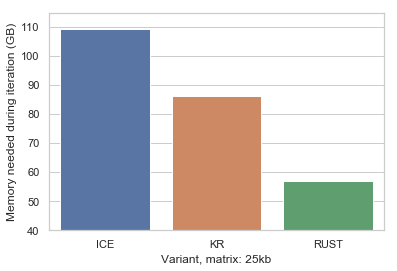
\includegraphics[scale=1]{figures/results/memiter_25}}
        \caption[Memory needs iterating 25kb]
        {\textbf{Memory needed during iteration} for correcting the 25kb matrix. Smaller is better.}
        \label{fig:memiter25}
\end{centering}
\end{figure}

\begin{figure}[t]
    \begin{centering}
        \subfloat[Available data]
        {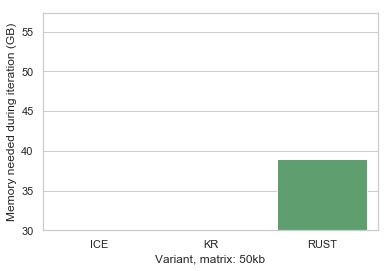
\includegraphics[scale=0.5]{figures/results/memiter_50}}
        \subfloat[Extrapolated data]
        {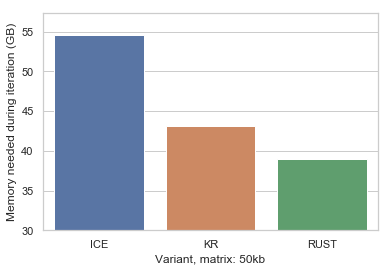
\includegraphics[scale=0.5]{figures/results/memiter_50_extra}}
        \caption[Memory needs iterating 50kb]
        {\textbf{Available and Extrapolated Data about Memory needed during
        iteration} of the 50kb matrix. Rust value is accurate, values for ICE
        and KR are not accurately available, but have been observed to be in
        the extrapolated areas. Smaller is better.}
        \label{fig:memiter50}
    \end{centering}
\end{figure}





\section{Memory Requirements}\label{sec:memory}

The memory requirements for these three algorithms are, or at least should be,
equal during loading, as the exact same code is executed. During loading,
memory was seen to fluctuate considerably, and was measured going up over 85
GByte at times. Initial loading time is proportional to matrix size, and
includes pre-processing. Prior to correction, zero values, \verb|NaN|s and
outliers are removed from the data. This needs between five and eight minutes
respectively (see \figref{fig:loadtimes} for reference).


\newpage
\subsection{During Correction}\label{sec:itermem}

Memory needs, at least for the iterative correction, have cycles. These cycles
correspond to the in \secref{sec:ICE} described steps, as the additional bias
matrices are not needed at any point other than for the correction itself. This
might be different for the implementation itself however, as e.g. in the Rust
implementation the memory needed for temporary biases is initialized before the
first iteration and is freed only after the last iteration finished.

A comparison of the three implementations regarding memory requirements during
correction of the 25kb connection matrix can be seen in \figref{fig:memiter25}.
As can be clearly seen, even though the recent KR implementation needs less
memory than the original ICE implementation, the new ICE implementation in Rust
needs even less, about half the amount the pure Python implementation needs.
Note that these are only comparisons of memory needs during iteration, there is
a different amount of memory needed for pre-processing and post-processing.

As can be seen in \figref{fig:memiter50}a, no reliable data except for the Rust
implementation exists for memory needs during computing of the 50kb matrix. In
\figref{fig:memiter50}b there is an extrapolation based on the data for the
25kb matrix and observed data, These values should not be taken at face value,
but they should not be too far off the truth. Here, the advantage of Rust
diminishes. Parts of the memory are still used from the initial pre-processing,
and the provided matrix itself (to the regarding algorithm) was only a copy.
Directly after loading (but before starting iteration), the needed memory when
correcting the 50kb matrix was 12GByte.


\subsection{Maximum required memory}\label{sec:maxmem}


\begin{figure}[!htbp]
    \begin{centering}
        \subfloat[Maximum resident set size when correcting 50kb matrix]
        {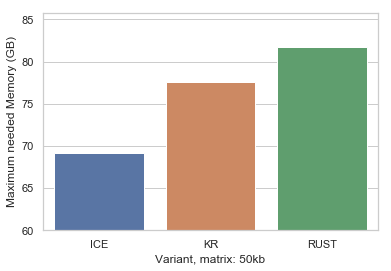
\includegraphics[scale=0.9]{figures/results/maxresident_50}} \\
        % \caption[Maximum needed Memory for 50kb]
        % {\textbf{Maximum needed Memory} when correcting the 50kb matrix.}
        \subfloat[Maximum resident set size when correcting 25kb matrix]
        {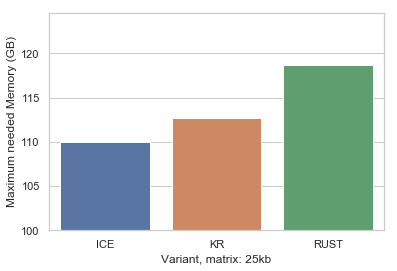
\includegraphics[scale=0.9]{figures/results/maxresident_25}}
        \caption[Maximum needed Memory]
        {\textbf{Maximum amount of needed Memory} when correcting 50kb and 25kb
        matrix. Smaller is better.}
        \label{fig:maxresident}
    \end{centering}
\end{figure}




Maximum required memory, or maxmimum resident set size, describes the highest
amount of memory needed at any point during execution. Maximum resident set size
is compared in \figref{fig:maxresident}.

After correction, the post-processing procedures differ. Both the Python and
C++ implementation return the corrected matrix as well as the correction
factors, while the Rust implementation is supposed to only return the
correction factors, as it does. This means that after returning the correction
factors, the corrected matrix from the rust part is not passed back, and a copy
of the original matrix is then corrected in Python again before saving the
corrected matrix.

When loading the matrix in the beginning, a considerable amount of working
memory is needed. However, the highest needs of memory are, at least for KR and
the RUST version, happening after the correction, when the corrected values are
set, the correction factors added and then saved. This might be due to
duplicate artifacts in memory, needing to be in memory in both Python and
the other language, while in the python version memory needs are considerably
lower during this process.

In Rust, indices are of type \verb|usize|, which size is platform-dependent. In
the case of the testserver (more details in \secref{sec:specs} and
\tabref{tab:specs}) this is the size of a \verb|int64|, whereas coming from
Python (and thus most likely in C++) it is only a \verb|int32|. Indices are a
considerable amount of memory in the case of a CSRMatrix, as there are more
indices than there are actual elements in the matrix, and the elements are only
of type \verb|float32|.

It is unclear if the RUST implementation (or the post-processing, since it is
different) would use more memory if available, as the needed memory was
supremely close to the actually available one. It is also unclear, if this
implementation would use less if less was available. The required memory could
most likely be reduced by returning the corrected matrix as well, or directly
correcting the original matrix within the memory from Python. This has been
deemed possible, as the CSRMatrix structure is build on top of \verb|numpy|
ndarrays implementation, with \verb|numpy| having a well documented C-API.





\subsection{Load times}\label{sec:loadtime}


\begin{figure}[!htbp]
    \begin{centering}
        \subfloat[Loading time in minutes for 25kb matrix]
        {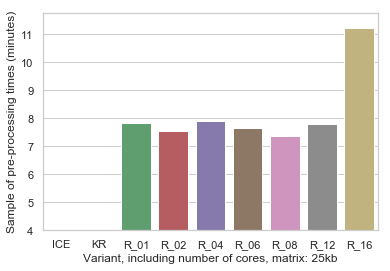
\includegraphics[scale=0.9]{figures/results/loadtimes_25}} \\
        % \caption[Correction time of 25kb]
        % {\textbf{Runtime in minutes} for correcting the 25kb matrix.}
        \subfloat[Loading time in minutes for 50kb matrix]
        {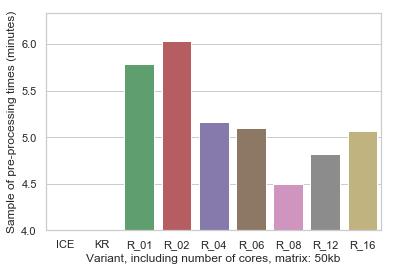
\includegraphics[scale=0.9]{figures/results/loadtimes_50}}
        \caption[Matrix loading times]
        {\textbf{Matrix loading times} for the different matrix sizes. Even though
        the operations are the same during pre-processing, actual times fluctuated.
        No data is available for ICE and KR variants, however as the pre-processing
        is the same, their values can be thought to be in the same range as the
        others. Equal is better.}
    \label{fig:loadtimes}
    \end{centering}
\end{figure}




Loading includes pre-processing the to-be corrected matrices. Pre-processing
steps include removal of zero-values, \verb|NaN|s from the dataset and
heavy outliers, as they would affect correction. However, even though the same
steps were performed in all cases, load times had significant outliers, as can
be seen in \figref{fig:loadtimes}. Here, loading times from seperate runs are
shown. The runs differ in that they were run in different configurations, which
start to differ after loading, as explained in more detail in
\secref{sec:multicore}. However as there is no difference up to this point,
they can very well be compared. Considering that there should no difference, it
is shocking to see that significant differences between loading times exist.

In the case of \figref{fig:loadtimes}a, most loading times are within half a
minute of each other, which could still be called deterministic considering the
size of the matrix and the amount of data written back and forth. The big jump
as seen in variant R\_16 however, should not be possible. Considering an
average time of around 7.5 minutes, 11.2 minutes are close to 50\% more than
that (49.4\%) ! This can only be described by the conditions of the virtual
server varying based on usage from other users, for which there is no data
available, except for deviations in this data, without knowledge what the
actual values would have been.

Loading times in \figref{fig:loadtimes}b do not differ by proportions as high,
but the clearly visible disparity is not something favourable.
% longest seen from the shortest is 33\% longer\footnote{(6 - 4.5) / 4.5
% = 33\%}, and the shortest is 25\% shorter when compared to the
% longest\footnote{(6 - 4.5) / 6 = 25\%}.


\subsection{Comparing Memory needs}\label{sec:compmemory}

\begin{table}[!htbp]
    \begin{tabular}{lrrr}
        \textbf{Overall memory comparison} & ICE & KR & RUST \\
        \midrule
        During iteration (50kb) &   54.6 & 43.1 & \textbf{39}   \\
        Maximum          (50kb) &   \textbf{69.2} & 77.6 & 81.7 \\
        During iteration (25kb) &   110 & 86 & \textbf{57}  \\
        Maximum          (25kb) &   \textbf{110} & 112.7 & 118.6 \\
    \end{tabular}
    \caption[Memory needs comparison]
    {\textbf{Overall comparison} between required memory for different
    situations. The ICE values for Maximum resident values are not considered,
    as they are probably wrong for some reason. See \secref{sec:maxmem} for
    details.}
    \label{tab:compmem}
\end{table}

As can be seen in \tabref{tab:compmem}, regarding memory usage each of the
algorithms has some advantage and another disadvantage. If working memory is a
critical resource, the question as to which is more critical, long-term lower
usage, or lower spike usage, becomes decisive for the selection of the
algorithm.




\section{Runtime length}\label{sec:runtime}


\begin{figure}[!htbp]
    \begin{centering}
        \subfloat[Runtime in minutes for correcting 25kb Matrix]
        {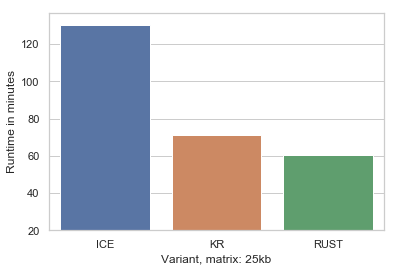
\includegraphics[scale=0.9]{figures/results/runtime_25}} \\
        % \caption[Correction time of 25kb]
        % {\textbf{Runtime in minutes} for correcting the 25kb matrix.}
        \subfloat[Runtime in minutes for correcting 50kb Matrix]
        {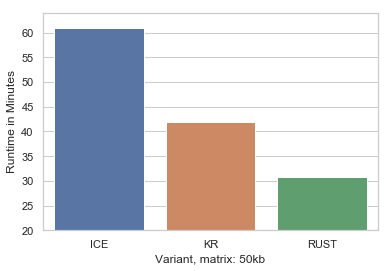
\includegraphics[scale=0.9]{figures/results/runtime_50}}
        \caption[Algorithm Runtimes]
        {\textbf{Algorithm Runtimes} for correcting the different matrices. It
        remains an open question why the difference between KR and RUST stays the
        same, even though both ICE and RUST double their computation time. Smaller
        is better.}
        \label{fig:runtime}
    \end{centering}
\end{figure}



In \figref{fig:runtime} a comparison of runtimes can be seen. The original
implementation in Python is taking the longest by a considerable amount, with
the implementation in Rust needing about half the time in both situations, less
than KR which is at only a third for 50kb. The difference itself, which is
about ten minutes, is roughly the same for both matrices though. In both cases
the difference is around ten minutes, whereas it is proportionally more when
the total runtime is only four times that amount versus ten minutes being only
a seventh of the total runtime, \figref{fig:runtime}b and \figref{fig:runtime}a
respectively.

An open question remains as to why this difference is roughly the same, even
though the python implementation needs about twice as much time, as does the
Rust one. It might be that the KR implementation is faster for considerably
bigger matrices. Testing this was not possible as the memory of the provided
virtual machine (see \secref{sec:specs} and \secref{sec:maxmem} for details)
did not allow loading of bigger matrices, and repeatedly failed trying to do
so.



\section{Multicore benefits}\label{sec:multicore}


\begin{figure}[!tbp]
\begin{centering}
    % \subfloat[Runtime in minutes for correcting 50kb Matrix]
    {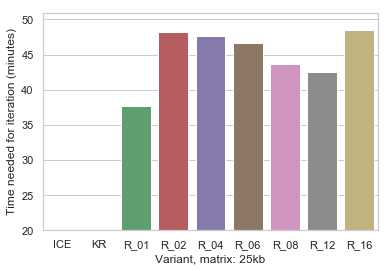
\includegraphics[scale=0.8]{figures/results/compute_multi_25}}
    \caption[Multicore comparison]
    {\textbf{Algorithm Runtimes} for correcting the different matrices. Smaller is better.}
    \label{fig:computetime25}
\end{centering}
\end{figure}




As can be seen in \secref{demo:par}, turning a single-core Rust program into
a multi-core program is not particularly difficult. Taking a look at
\figref{fig:computetime25}, the advantage of using multiple cores is everything
but apparent, in fact it is even slower than not using it. There are multiple
reasons for this. First, most of the parallelized operations are considerably
small, sometimes just slightly more complex than a list summation. In the case
of parallelizing list summations as well, total runtime becomes similar to the
original ICE implementation, as there are several summations for each
iteration. Even though the operations themselves are rather small, the overhead
for how to distribute them is still added, even in the case of using only one
core. This overhead is spreaded across several cores as well, but even using 12
cores is not sufficient for amortizing the additional overhead. The scheduler
of \verb|rayon|, the used library for this, is a work-stealing scheduler,
meaning that initially every thread in the threadpool gets a roughly equal
amount, and as soon as one core is done earlier than the others, its stealing
work from other cores. Initially all work is distributed over the available
threads in chunks. This initial distribution makes up a significant amount of
overhead. In the case of 16 Threads (and above in cases tested), the main
overhead is coming from too many threads having finished earlier and stealing
work from each other.

Even though the current version does support parallelization, it does not
provide benefits. They might only visualize for even bigger matrices, where the
amount of needed work amortizes the initial overhead better. Additionally,
there is more potential for combining operations for parallelization. For some,
this is clearly not possible, but for several it would be possible to combine
them, reducing the overhead for parallelization at one point, and parallelizing
heavier operations instead.


\begin{figure}[!htbp]
    \begin{centering}
        \subfloat[Memory needed during iteration when correcting 25kb matrix]
        {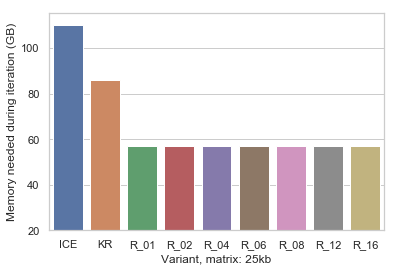
\includegraphics[scale=0.5]{figures/results/memiter_multi_25}}
        \subfloat[Maximum resident set size when correcting 25kb matrix]
        {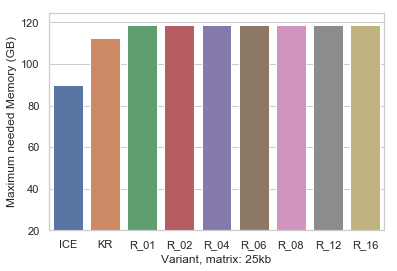
\includegraphics[scale=0.5]{figures/results/maxresident_multi_25}}
        \caption[Multicore Memory comparison]
        {\textbf{Multicore Memory needs} for correcting the 25kb matrix. Memory
        needs stay the same in all versions. Based on the numbers, there is no
        difference between the single-core version and any multi-core version
        regarding memeory usage.}
        \label{fig:memmulti}
    \end{centering}
\end{figure}


\begin{figure}[!htbp]
    \begin{centering}
        % \subfloat[subfloat-text]
        {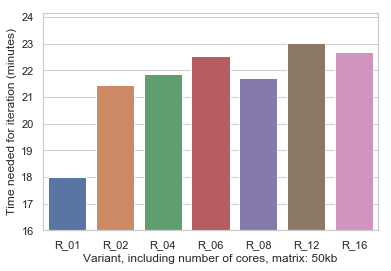
\includegraphics[scale=0.8]{figures/results/runtime_multi_50}}
        \caption[Multi-core computation time comparison]
        {\textbf{Multi-core computation time comparison} for 50kb matrix. These are
        pure computing times, excluding both pre- and post-processing. No numbers
        for ICE and KR are available. Smaller is better.}
        \label{fig:mrun50}
    \end{centering}
\end{figure}


However, as can be seen in \figref{fig:memmulti}, memory is not negatively
affected in any way when parallizing. Regarding memory, the same holds true for
the 50kb matrix. Pure computation times for the 50kb matrix as seen in
\figref{fig:mrun50} do not seem to offer a clear trend regarding the usage of
multiple cores.


\paragraph{Conclusion:} Using multiple cores for this implementation does not
provide any benefit, however it does have significant downsides other than
longer runtime. The algorithm may be rewritten to allow better multicore usage.



\section{Output}

\begin{figure}[!htbp]
    \begin{centering}
        \subfloat[original values]{
            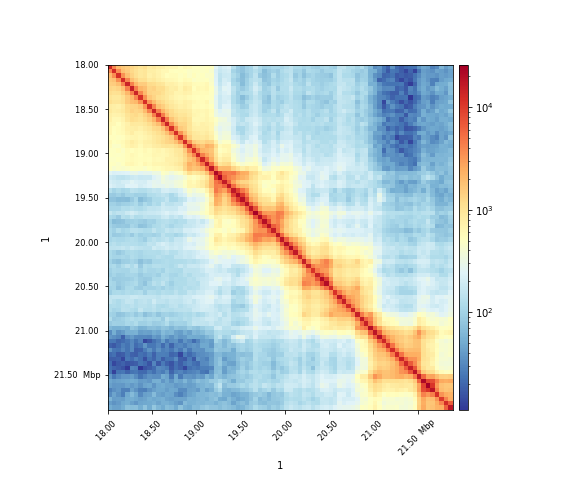
\includegraphics[scale=0.4]{figures/results/c_50kb}}
        \subfloat[RUST]{
            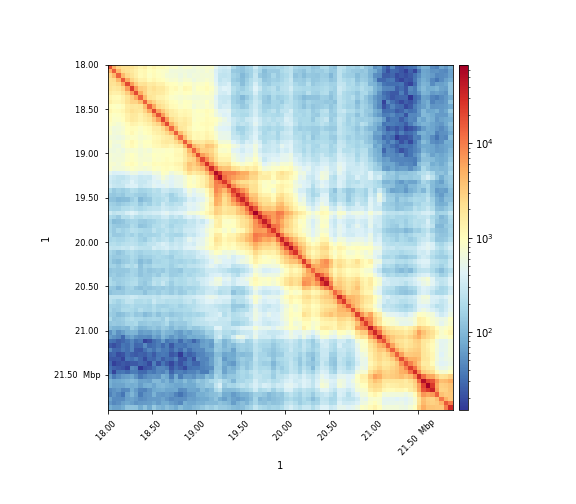
\includegraphics[scale=0.4]{figures/results/c_rust_50kb}} \\
        \subfloat[ICE]{
            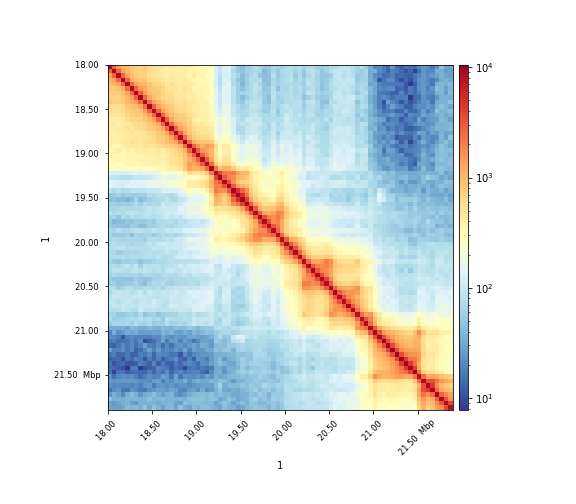
\includegraphics[scale=0.4]{figures/results/c_ice_50kb}}
        \subfloat[KR]{
            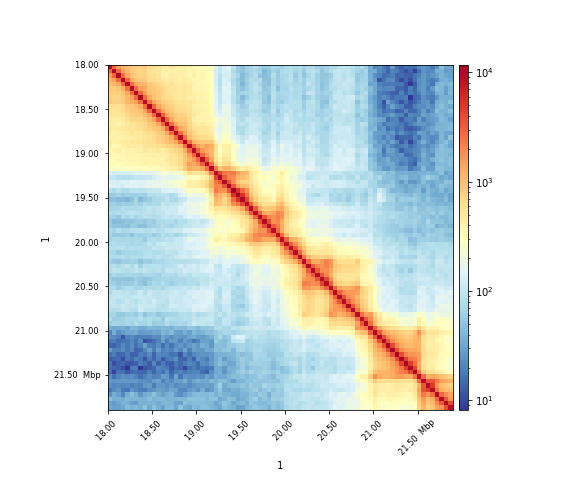
\includegraphics[scale=0.4]{figures/results/c_kr_50kb}}
        \caption[Plotting corrected matrices]
        {\textbf{Original and corrected matrices.} In \textbf{(b)} there appear to be
        higher maximum values, setting the cutoff lower creates pictures
        undistinguishable to those from ICE or KR.
        Images were created using hicPlotMatrix.
        }
        \label{fig:plotted}
    \end{centering}
\end{figure}


One essential point of a reimplementation is the correctness of of the output.
As can be seen in \figref{fig:plotted}, the output from both the original ICE
implementation and the KR version are pretty much the same. The output of the
RUST implementation is closer to the original values however. Due to time
contraints the differences between the output matrix in the Rust implementation
could not be further explored, but are likely due to different thresholds in
the implementation of the algorithm.





% using hicPlotMatrix -m <matrixname> --region 1:18000000-22000000 --log1p -o <outfile>.png


    \chapter{Conclusions}\label{chap:conclusion}


\section{Comparing the Different Implementations}

\paragraph{Memory and Runtime:}
Both Memory needs and Runtime length have been discussed extensively in
\secref{sec:memory} and \secref{sec:runtime} respectively. Comparisons can be
seen in \tabref{tab:compmem} for memory and \figref{fig:runtime} for runtime.
In short: the new ICE implementation in Rust requires considerably less memory
than the Python implementation during correction. After the correction, it
peaks at a slightly higher value than the Python implementation requires at any
point in time. KR is in the middle for both, memory-wise. Additionally, the new
implementation requires only about half the runtime length compared to the
Python implementation, beating KR by about 10 minutes in both test cases.


\paragraph{Unused Potential:}\label{sec:potential} This includes the further
optimization of both the C++ and Rust versions, and increasing their level of
integration. Apparently, a revision of the KR implementation is in progress,
needing considerably less memory for bigger matrices. The Rust version could be
revised to make more effective use of opportunities for parallelization, and
integrated better in the Python part in order to reduce peak memory usage
tremendously.


\paragraph{Overall:} Each of the current implementations has their own
advantages and disadvantages, providing more flexibility for adapting to
differently constrained resource environments.


\section{Python interacting with Rust:} Even though there have been
difficulties for getting the code packaged, it worked surprisingly well after
this was fixed. There is still work ongoing to make Rust usage from Python
considerably easier. It is well needed, as there is not one standard
approach but several partially similar, but exclusive ones.

The approach recommended by the official Rust Book turned out to be not as easy
as expected regarding packaging. However, two other common approaches make
significant promises regarding this. Thus, it is probably easier to package
Rust code for Python using either one of the two other integration approaches
described in \secref{sec:api}.

\textbf{Overall, more extensive testing for integration approaches is recommended.}


\section{Open questions}

One of the biggest remaining open questions is regarding the more effective use
of multi-core hardware, as to how much it would be possible to actually do
this, in Rust or any other language, and how much of a benefit it would bring.
Both the pre-processing and post-processing mainly use only one core during
their execution. Some of it may not at all be parallelizable, but there are
probably several low-hanging fruits regarding optimization.

Other questions are regarding the currently unused potential mentioned in
\secref{sec:potential}, particularly the closer integration from within Python,
as it would directly affect memory requirements. A pure implementation in
either C++ or Rust is likely to need less memory than when integrated with
Python, based on the numbers and the reasons for the numbers seen in
\secref{sec:maxmem} about peak memory usage.

Based on available data, the available resources are far from sufficient for
comparing runtimes of considerably bigger matrices (see \secref{sec:specs} for
available resources, and \secref{sec:data} for data about the compared
matrices).
However, with sufficient resources at least this open question could be
answered: For the biggest matrices, is KR still only the second fastest, or
will it actually be faster and more memory efficient than this implementation?









% \newpage


% \todo{clean up GitHub and add documentation (on last day)}
% 
% 
% \todo{make sure everything is cited appropriately!}
% 
% \todo{make sure everything is cited appropriately!}
% 
% \todo{make sure everything is cited appropriately!}

% \todo{Let the number of references become 30!}



% For presentation:

% \todo{for presentation: 1/3 for everyone, 1/3 for supervisor + experts, 1/3 only I am expert}

% \todo{biggest points: Python to rust and how it worked, give code examples but not too much}


    \chapter{Acknowledgments}

First and foremost, I would like to thank...
\begin{itemize}
\item{advisers}
\item{examiner}
\item{person1 for the dataset}
\item{person2 for the great suggestion}
\item{proofreaders}
\end{itemize}

    % If you want a list of your ToDos at the end of the document
    % don't forget to remove before submission!
    % place it somewhere in the document
\chapter*{ToDo Counters}
\newcounter{ct}%
To Dos: \arabic{todos}; \hspace{1em}%
\setcounter{ct}{0}%
\whiledo {\value{ct} < \value{todos}}%
{%
	\stepcounter {ct}%
    \ref{todo \thect}%
	\ifnum\value{ct} = \value{todos}{}\else{, }\fi
}

Parts to extend: \arabic{extends}; \hspace{1em}%
\setcounter{ct}{0}%
\whiledo {\value{ct} < \value{extends}}%
{%
	\stepcounter {ct}%
	\ref{extend \thect}%
	\ifnum\value{ct} = \value{extends}{}\else{, }\fi
}

Draft parts: \arabic{drafts}; \hspace{1em}%
\setcounter{ct}{0}%
\whiledo {\value{ct} < \value{drafts}}%
{%
	\stepcounter {ct}%
	\ref{draft \thect}%
	\ifnum\value{ct} = \value{drafts}{}\else{, }\fi
}


    \bibliographystyle{ieeetr}
    \bibliography{bib/references.bib}
    % bibliography is not in the table of contents per default, add it manually
    % enable the \renewcommand for german header
    % \renewcommand{\bibname}{Literaturverzeichnis}

    \addcontentsline{toc}{chapter}{Bibliography}
    \newpage
    \thispagestyle{empty}
    \mbox{}


\end{document}
